\documentclass{article}
\usepackage[utf8]{inputenc}

\title{EE2703 Applied Programming Lab \\   Assignment 8 \\  Digital Fourier Transform}  
\author{
  \textbf{Name}: Neham Hitesh Jain\\
  \textbf{Roll Number}: EE19B084
}\date{April 23, 2021}

\usepackage{listings}
\usepackage{natbib}
\usepackage{geometry} % Used to adjust the document margins
\usepackage{amsmath}
\usepackage{subfig}
\usepackage{verbatim}
\usepackage{color}
\usepackage{graphicx}
\definecolor{dkgreen}{rgb}{0,0.5,0}
\definecolor{gray}{rgb}{0.5,0.5,0.5}
\definecolor{mauve}{rgb}{0.58,0,0.82}

\lstset{frame=tb,
  language=Python,
  aboveskip=3mm,
  belowskip=3mm,
  showstringspaces=false,
  columns=flexible,
  basicstyle={\small\ttfamily},
  numbers=none,
  numberstyle=\tiny\color{gray},
  keywordstyle=\color{blue},
  commentstyle=\color{dkgreen},
  stringstyle=\color{mauve},
  breaklines=true,
  breakatwhitespace=true,
  tabsize=3
}

\geometry{verbose,tmargin=1in,bmargin=1in,lmargin=1in,rmargin=1in}

\begin{document}

\maketitle
\newpage

\begin{abstract}
    This week’s assignment deals with analysing signals using the Fast Fourier
    Transform(FFT) using the numpy’s fft module. The FFT is a fast implementation of 
    the Discrete Fourier transform(DFT). We also attempt to approximate the CTFT 
    of a Gaussian by changing the window size and number of samples until 
    the error is below a threshold.    

\end{abstract}

\section*{FFT and IFFT}\label{fft-and-ifft}

We perform the FFT and then the IFFT on a random array to see how well
the original signal can be reconstruced.

\begin{lstlisting}

#Example 1
x=rand(100)
X=fft(x)
y=ifft(X)
c_[x,y]
print ("The Absolute Maximum Error is ",abs(x-y).max())

\end{lstlisting}

\begin{verbatim}
Maximum absolute error in reconstruction: 4.417237552752643e-16    
\end{verbatim}

An error of order \(10^{-16}\) is present due to numerical inaccuracies
in representations. We also observe that the reconstructed signal has
some very small imaginary parts. Otherwise, we can see that the
reconstruction is almost perfect.



\section*{Spectrum of $sin(5t)$}
The solution for this is already a part of the assignment. 
As expected the phase fro some values near the peaks is non zero. 
To fix this we sample the input signal at an appropriate frequency. 
We also shift the phase plot so that it goes from $-\pi$ to $\pi$. 
To do this we write a helper function.  \\

\noindent
The phase of the points which significant magnitude values are denoted by green coloured scatter points


\begin{lstlisting}
def estimate_dft(func_name,x_start,x_end,steps,
xlim1,title1,title2,ylabel1,ylabel2,xlabel1,savename,ro,ylim):
    
    sampling_rate = steps/(x_end-x_start)
    x=linspace(x_start,x_end,steps+1)[:-1]
    y = func_name(x)
    Y=fftshift(fft(y))/float(steps)
    w=sampling_rate*(linspace(-pi,pi,steps+1)[:-1])
    
    p1=General_Plotter(xlabel1,ylabel1,ylabel2,title1,title2,savename)
    p1.plot_fft(w,Y,scatter=True,ro=ro,xlim=xlim1,ylim=ylim)

\end{lstlisting}

As expected we get 2 peaks at +5 and -5 with height 0.5. 
The phases of the peaks at $\frac{\pi}{2}$ and $-\frac{\pi}{2}$ are also expected based as the expansion of a sine wave ie:

\begin{equation}
sin(5t) = 0.5(\frac{e^{5t}}{j}-\frac{e^{-5t}}{j})
\end{equation}

\begin{figure}[!tbh]
\centering
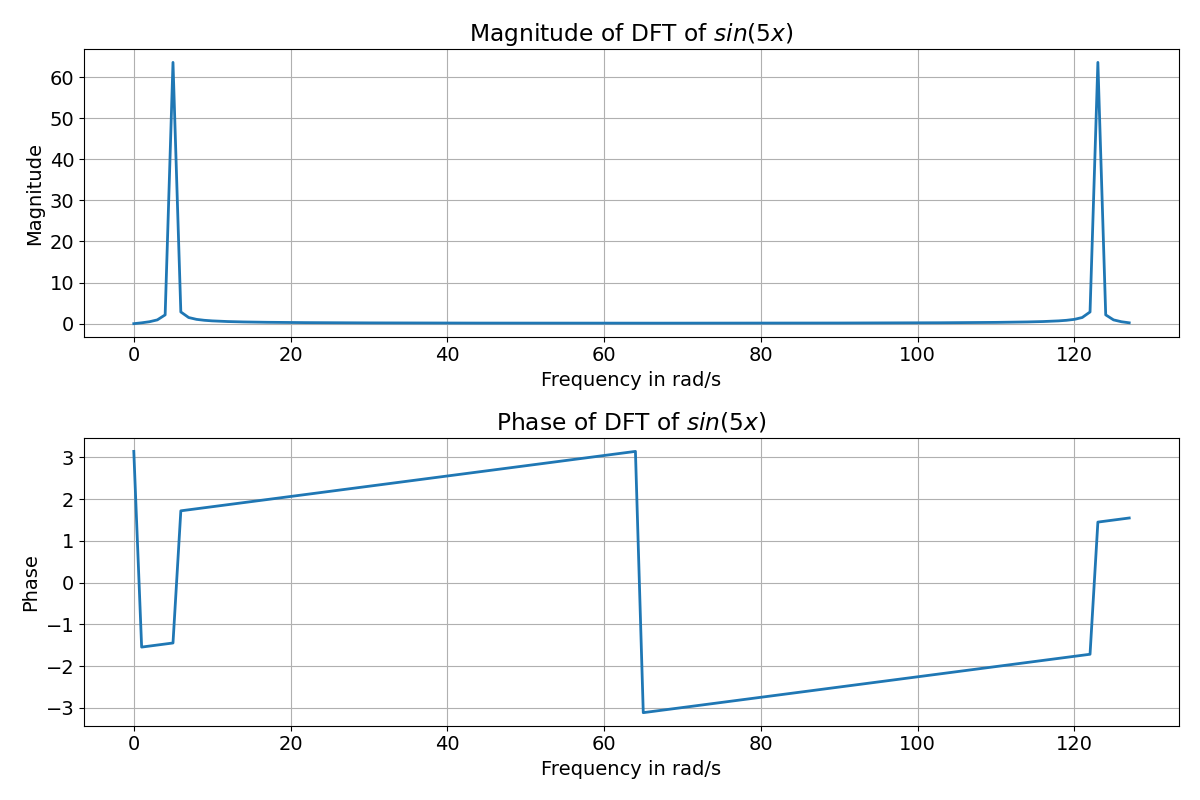
\includegraphics[scale=0.4]{plots/fft_unshifted_sin(5x).png}
\caption{Spectrum of unshifted form of $sin(5t)$ }
\label{fig:1}
\end{figure}
\newpage
\begin{figure}[!tbh]
\centering
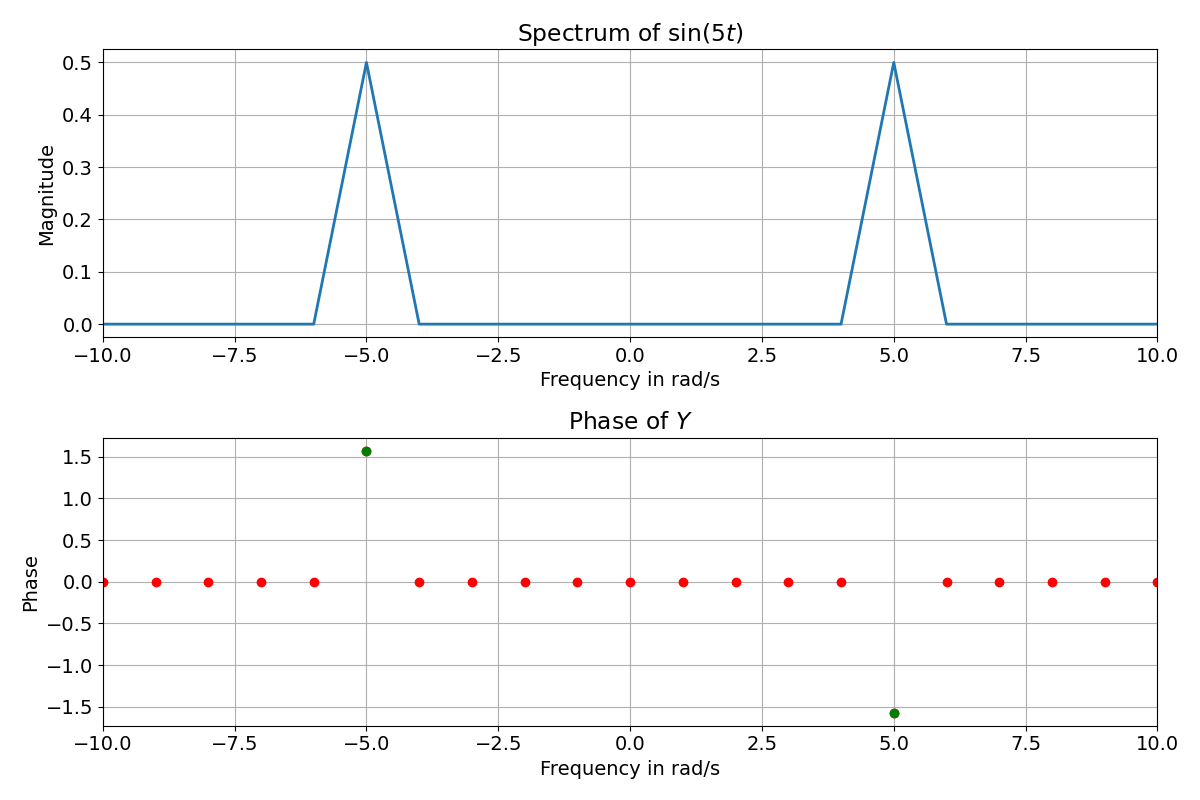
\includegraphics[scale=0.4]{plots/sin(5x)_shifted.png}
\caption{Spectrum of shifted form of $sin(5t)$}
\label{fig:2}
\end{figure}

\section*{Spectrum of Amplitude Modulated Wave}
Consider the signal:\newline
\begin{equation}
f(t) = (1+0.1\cos(t))\cos(10t)    
\end{equation}
Using the same function as before, we get the following output:
\begin{figure}[!tbh]
\centering
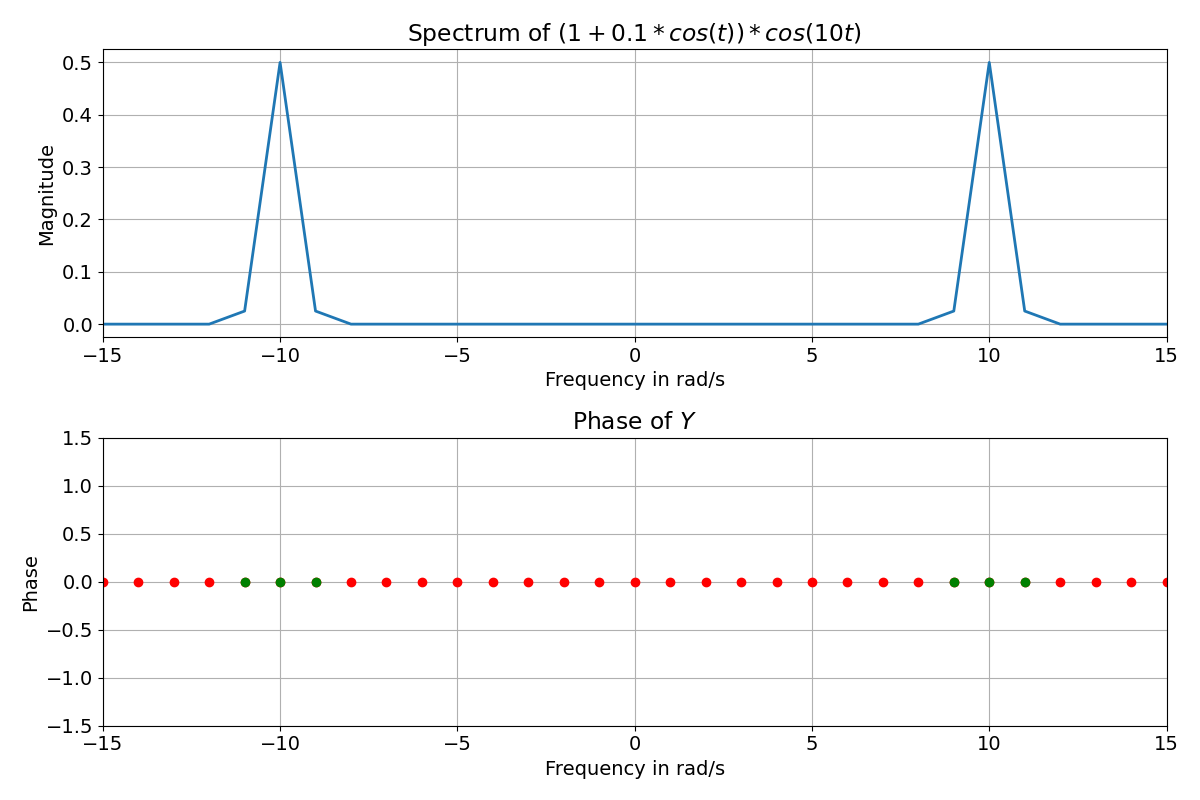
\includegraphics[scale=0.4]{plots/1+cos(0.1t).png}
\caption{Spectrum of $f(t) = (1+0.1\cos(t))\cos(10t)$ with low number of samples}
\label{fig:3}
\end{figure}
\newpage
We note that 2 of the peaks have merged, we need to increase the number of samples we take. Calling the same function with a larger range and a higher number of samples we get 3 peaks. At all 3 peaks, the phase is 0 as expected for a cosine wave.
\begin{figure}[!tbh]
\centering
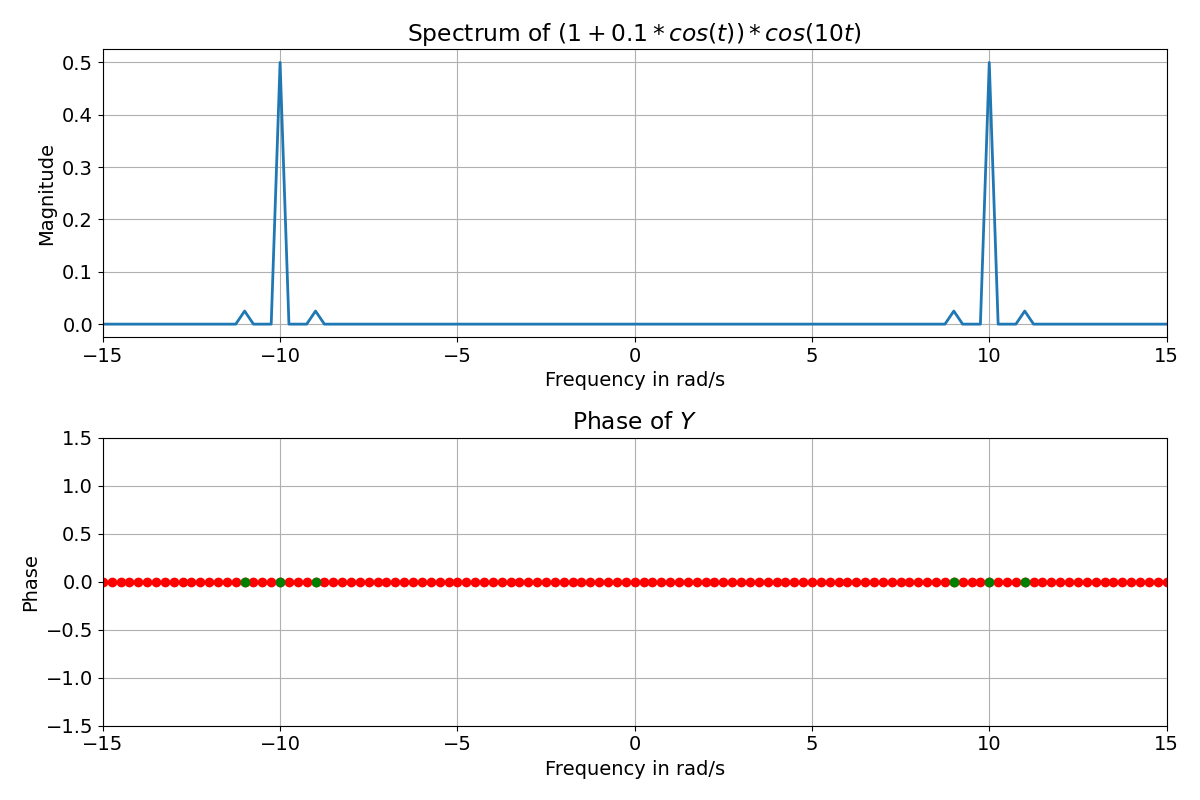
\includegraphics[scale=0.45]{plots/1+cos(0.1t)_stretched.png}
\caption{Spectrum of $f(t) = (1+0.1\cos(t))\cos(10t)$ with a higher number of samples}
\label{fig:4}
\end{figure}

\section*{Spectrum of $sin^3(t)$}
This signal can be expressed as a sum of sine waves using this identity:\newline

$\sin^3(t) = \frac{3}{4}\sin(t) - \frac{1}{4}\sin(3t)$\newline

\noindent
We expect 2 peaks at frequencies 1 and 3, and a phase angle similar to that expected from a sum of sinusoids.
\begin{figure}[!tbh]
\centering
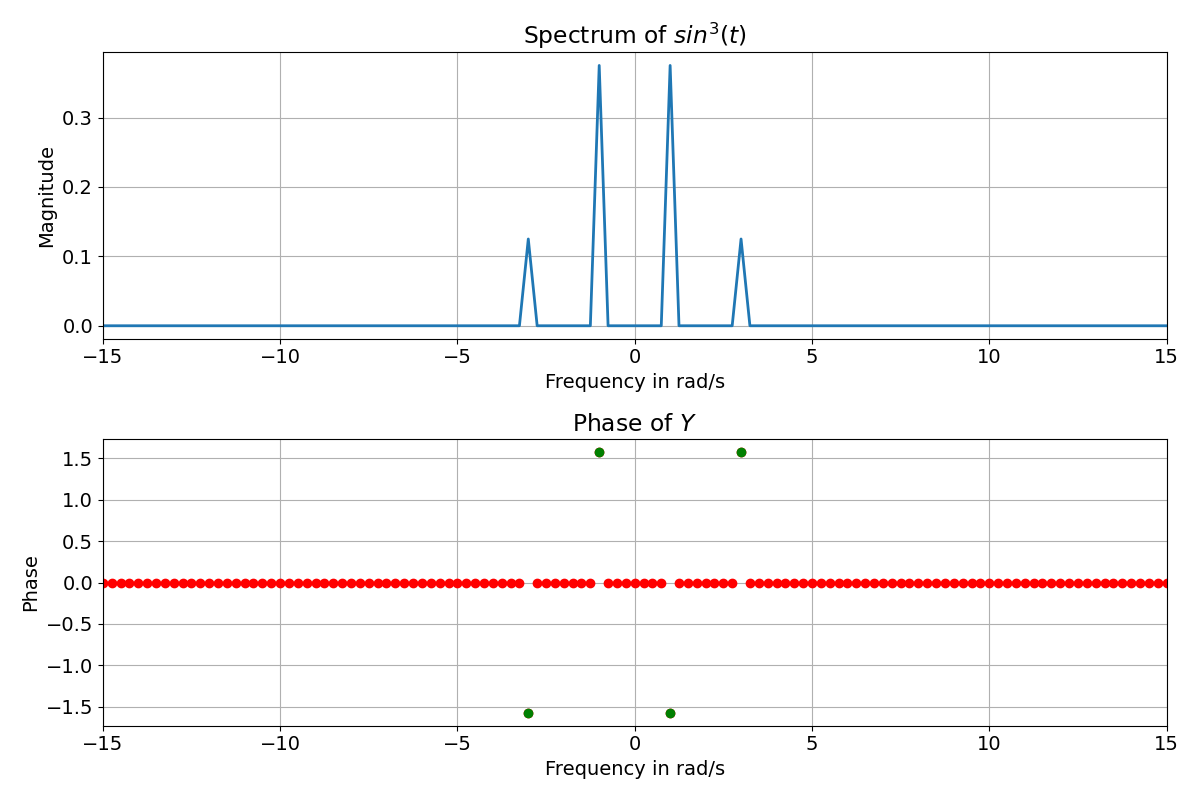
\includegraphics[scale=0.4]{plots/sin3.png}
\caption{Spectrum of $f(t) = sin^3(t)$}
\label{fig:5}
\end{figure}

\section*{Spectrum of $cos^3(t)$}
This signal can be expressed as a sum of cosine waves using this identity:\newline

$\sin^3(t) = \frac{3}{4}\cos(t) + \frac{1}{4}\cos(3t)$\newline

\noindent
We expect 2 peaks at frequencies 1 and 3, and phase=0 at the peaks.

\begin{figure}[!tbh]
\centering
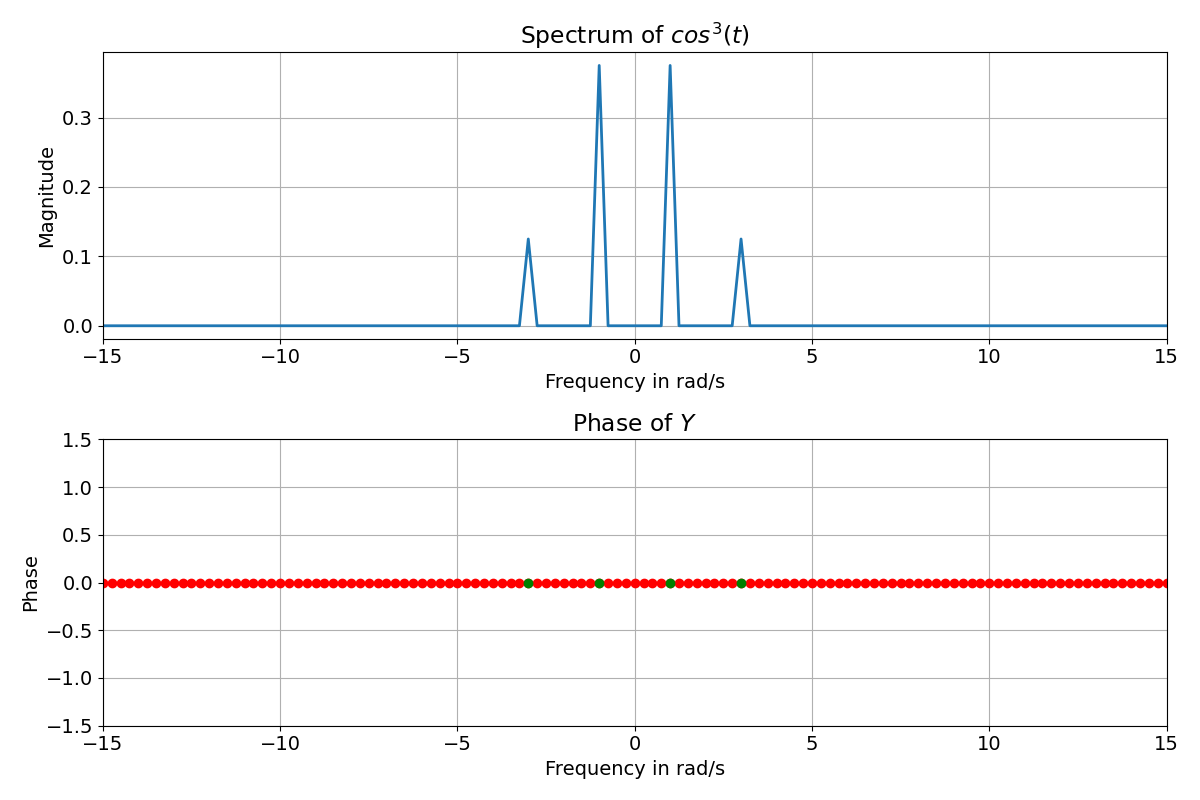
\includegraphics[scale=0.4]{plots/cos3.png}
\caption{Spectrum of $f(t) = cos^3(t)$}
\label{fig:6}
\end{figure} 

\section*{Spectrum of Frequency Modulated Wave}
Consider the signal:\newline
\begin{equation}
f(t) =  \cos(20t +5 \cos(t))    
\end{equation}

Using the same helper function as before, we get the following output:\newline
\begin{figure}[!tbh]
\centering
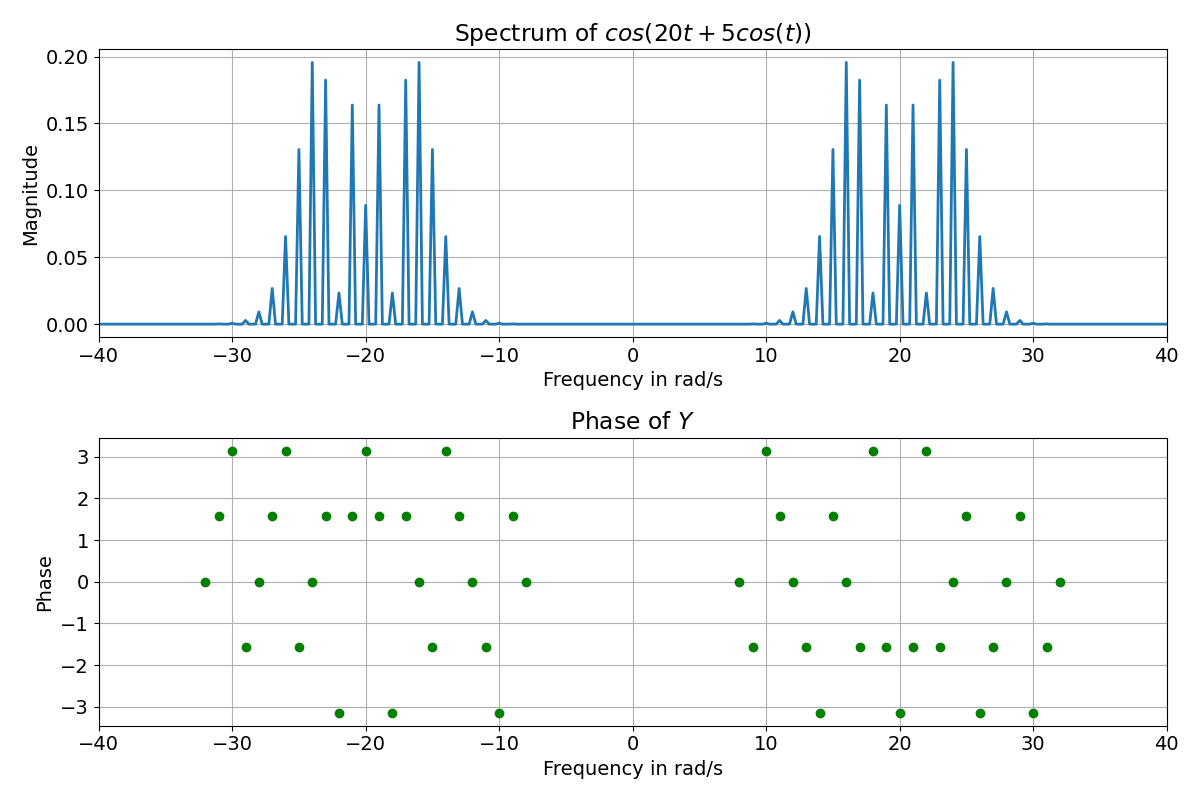
\includegraphics[scale=0.4]{plots/freq_mod.png}
\caption{Spectrum of $f(t) = (1+0.1\cos(t))\cos(10t)$}
\label{fig:7}
\end{figure}

The number of peaks has clearly increased. The energy in the side bands is comparable to that of the main signal.



\section*{Continuous time Fourier Transform of a Gaussian}
		
The Fourier transform of a signal $x(t)$ is defined as follows:\newline
\begin{equation}
X(\omega) = \frac{1}{2 \pi} \int_{- \infty}^{\infty} x(t) e^{-j \omega t} dt    
\end{equation}

\noindent
We can approximate this by the Fourier transform of the windowed version
of the signal $x(t)$, with a sufficiently large window as Gaussian curves tend to $0$ for large values of $t$ . Let the window be of size $T$. We get:

\begin{equation}
  X(\omega) \approx \frac{1}{2 \pi} \int_{- T/2}^{T/2} x(t) e^{-j \omega t} dt  
\end{equation}

\noindent
On writing the integral as a Riemann sum with a small time step $\Delta t = \frac{T}{N}$, We get:

\begin{equation}
    X(\omega) \approx \frac{\Delta t}{2 \pi} \sum_{n = -\frac{N}{2}}^{\frac{N}{2}-1} x(n \Delta t) e^{-j \omega n \Delta t}
\end{equation}

\noindent
Now, we sample our spectrum with a sampling period in the frequency
domain of \(\Delta \omega = \frac{2 \pi}{T}\), which makes our
continuous time signal periodic with period equal to the window size
\(T\). Our transform then becomes:

\begin{equation}
X(k \Delta \omega) \approx \frac{\Delta t}{2 \pi} \sum_{n = -\frac{N}{2}}^{\frac{N}{2}-1}x(n \Delta t) e^{-j \frac{2 \pi}{N} k n} 
\end{equation}

\noindent
This form is similar to a DFT(for a finite window size). Therefore:
\begin{equation}
X(k \Delta \omega) \approx \frac{\Delta t}{2 \pi} DFT \{x(n \Delta t)\}    
\end{equation}

\noindent
We made a few approximations by using a finite window size and by using the Riemann approximation \\

\noindent
We can improve these approximations by making the window size $T$ larger, and by 
decreasing the time domain sampling period or increasing the number of samples $N$. 
We find the appropriate values for these iterative keeping the sampling frequency constant. \\

\noindent
The expression for the Gaussian is :

\begin{equation}
    x(t) = e^{\frac{-t^2}{2}}    
\end{equation}
The CTFT is given by:
\begin{equation}
X(j \omega) = \frac{1}{\sqrt{2 \pi}}e^{\frac{-\omega^2}{2}}    
\end{equation}
\begin{lstlisting}

def estimateCTFT(func, tol=1e-6,time_samples=128, true_func=None,func_name=None, wlim=None, scatter_size=40):
    """Estimate the continuous time Fourier Transform of the given function
    by finding the DFT of a sampled window of the function. The magnitude and
    phase of the estimate are also plotted.
    
    """
    T = 8*pi
    N = time_samples
    Xold = 0
    error = tol+1
    iters=0
    
    while error>tol:
        
        delta_t = T/N # time resolution
        delta_w = 2*pi/T # frequency resolution

        W = N*delta_w # total frequency window size

        t = linspace(-T/2,T/2,N+1)[:-1] # time points
        w = linspace(-W/2,W/2,N+1)[:-1] # freq points

        x = func(t)

        # find DFT and normalize
        # note that ifftshift is used to prevent artifacts in the
        # phase of the result due to time domain shifting
        X = delta_t/(2*pi) * fftshift(fft(ifftshift(x)))
        
        error = sum(abs(X[::2]-Xold))
        
        Xold = X
        N *= 2 # number of samples
        T *= 2 # total time window size
        iters+=1
        
    print("DTFT Approximation Results:")    
    print("Estimated error after {} iterations: {}".format(iters, error))
    print("Time range : ({:.4f}, {:.4f})".format(-T/2,T/2))
    print("Time resolution : {:.4f}".format(delta_t))
    print("Frequency resolution : {:.4f}".format(delta_w))
        
    if true_func != None:
        true_error = sum(abs(X-true_func(w)))
        print("True error: {}".format(true_error))
    
    mag = abs(X)
    ph = angle(X)
    ph[where(mag<tol)]=0
    #Magnitude
    p1=General_Plotter("Frequency in rad/s","Magnitude",r"Phase",r"Magnitude of CFT Estimate of $e^{\frac{-t^2}{2}}$",r"Phase of CFT Estimate","CFT_Estimate")
    p1.plot_fft(w,mag*np.exp(1j*ph),scatter=True,ro=True,xlim=wlim)
    
    X_ = true_func(w)    
    mag = abs(X_)
    ph = angle(X_)
    ph[where(mag<tol)]=0
    
    p2=General_Plotter("Frequency in rad/s","Magnitude",r"Phase",r"Magnitude of True CFT of $e^{\frac{-t^2}{2}}$",r"Phase of True CFT","True_CFT")
    p2.plot_fft(w,mag*np.exp(1j*ph),scatter=True,ro=True,xlim=wlim)

\end{lstlisting}

\begin{figure}[!tbh]
\centering
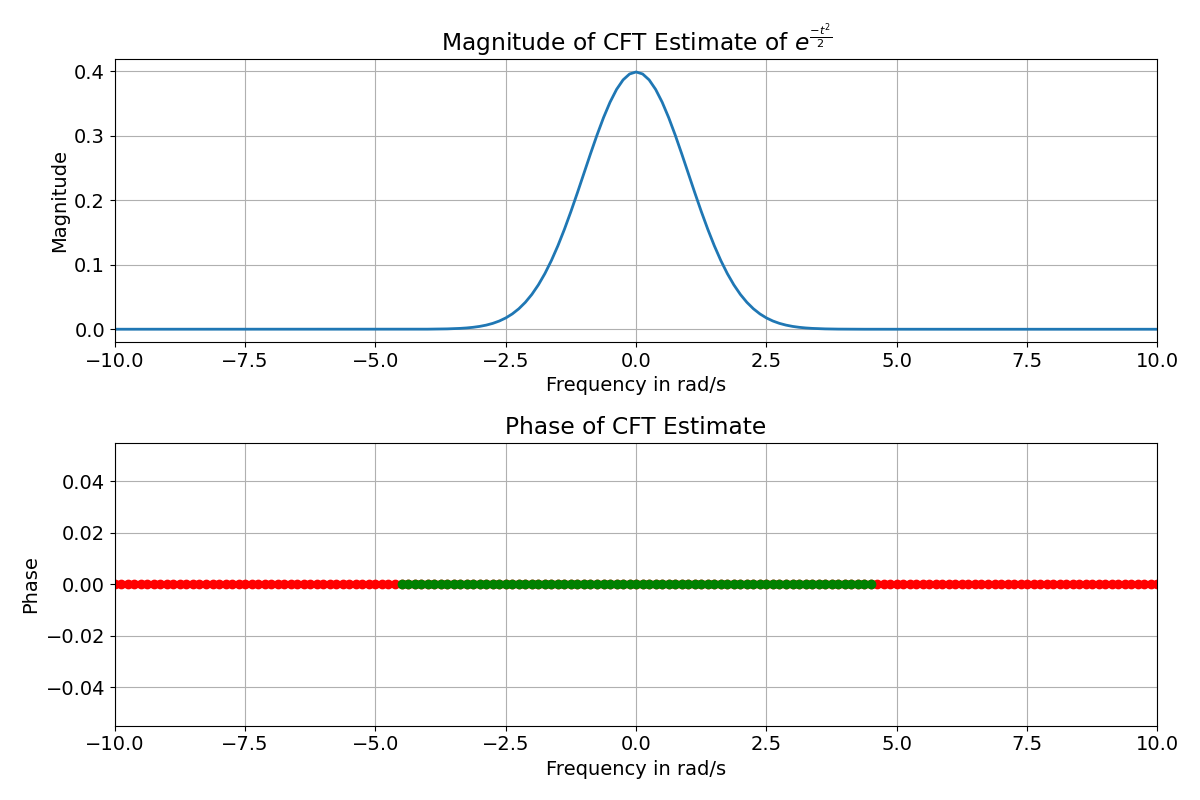
\includegraphics[scale=0.4]{plots/CFT_Estimate.png}
\caption{Estimated Continuous Time Fourier Transform of a Gaussian}
\label{fig:8}
\end{figure}

\begin{figure}[!tbh]
\centering
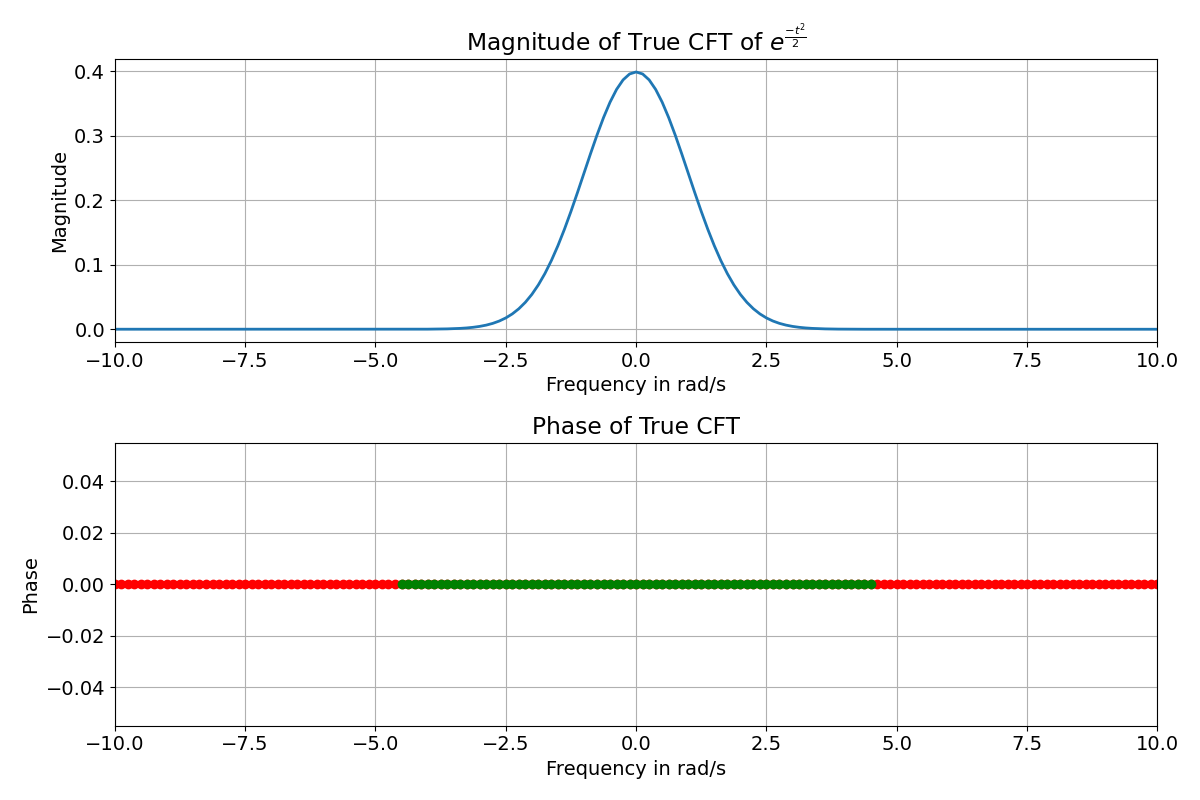
\includegraphics[scale=0.4]{plots/True_CFT.png}
\caption{Expected Continuous Time Fourier Transform of a Gaussian}
\label{fig:9}
\end{figure}

\newpage
		
\section*{Conclusions}\label{conclusions}

\begin{itemize}
\item
  From the above pairs of plots, it is clear that with a sufficiently
  large window size and sampling rate, the DFT approximates the CTFT of
  the Gaussian.
\item
  This is because the magnitude of the Gaussian quickly approaches \(0\)
  for large values of time. This means that there is lesser frequency
  domain aliasing due to windowing. This can be interpreted as follows:
\item
  Windowing in time is equivalent to convolution with a sinc in
  frequency domain. A large enough window means that the sinc is tall
  and thin. This tall and thin sinc is approximately equivalent to a
  delta function for a sufficiently large window. This means that
  convolution with this sinc does not change the spectrum much.
\item
  Sampling after windowing is done so that the DFT can be calculated
  using the Fast Fourier Transform. This is then a sampled version of
  the DTFT of the sampled time domain signal. With sufficiently large
  sampling rates, this approximates the CTFT of the original time domain
  signal.
\item
  This process is done on the Gaussian and the results are in agreement
  with what is expected.
\end{itemize}



\end{document}